\subsection{Modelo predictivo}
\label{cap:EstimacionVelocidad}

En esta sección se describe la metodología utilizada para crear un proceso o modelo el cual es utilizado para determinar la velocidad de vehículos. Se implementaron dos procesos para esta tarea. El primer proceso utiliza la fórmula física de la velocidad, a partir de esta fórmula se busca un factor de correlación entre la distancia en píxeles recorrida por el vehículo y la distancia en metros. Mientras que el segundo proceso implementado usa un modelo de aprendizaje máquina utilizando bibliotecas de Python las cuales ayudan a crear un modelo predictivo con el cual se determina la velocidad del vehículo.

\subsubsection{Estimar velocidad basado en factor de correlación}
\label{cap:EstimarVelocidadBasadoFactorCorrelacion}
Para determinar la velocidad utilizando el conjunto de datos generado por el sistema se inicia utilizando la fórmula física descrita en la Ecuación \ref{eq:Velocidad} para el cálculo de la velocidad.

\begin{equation}
    \label{eq:Velocidad}
    Velocidad = \frac{Distancia}{Tiempo}
\end{equation}

En este caso las muestras fueron tomadas por un Radar que solo proporciona la velocidad en Kilómetros o en Millas, así que necesitamos convertir este valor a metros sobre segundo, utilizando la Ecuación \ref{eq:ConvertMSKH}.

\begin{equation}
    \label{eq:ConvertMSKH}
    \frac{M}{S} = \frac{18}{5} \times \frac{K}{H}
\end{equation}

A partir de la Ecuación \ref{eq:Velocidad} donde se realiza cálculo de la velocidad y la conversión de la velocidad en metros por segundo en lugar de kilómetros por hora. La Figura \ref{fig:CrearModeloCustom} define los pasos que se deben seguir para modelar los datos obtenidos utilizando un factor de correlación.
Se define el proceso para crear el modelo en el diagrama de flujo que se muestra en la Figura \ref{fig:CrearModeloCustom}.

\begin{figure}[H]
    \centering
    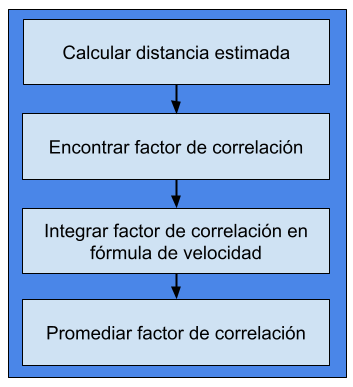
\includegraphics[width=0.5\textwidth]{Metodologia/imgs/DFCrearModeloCustom.png}
    \caption{Diagrama de flujo para la creación de modelo con la fórmula física de la velocidad.}
    \label{fig:CrearModeloCustom}
\end{figure}

La Tabla \ref{tab:CaracteristicasSistema} muestra que los tres parámetros necesarios para estimar la velocidad, sin embargo, el valor de la distancia está en pixeles, por lo que es necesario convertir el valor a metros. Este valor es convertido con la Ecuación \ref{eq:Velocidad} despejando la distancia, obteniendo la  Ecuación \ref{eq:DistanciaEstimada}.

\begin{equation}
    \label{eq:DistanciaEstimada}
    Distancia\:Estimada = Tiempo \times Velocidad
\end{equation}

Una vez que se tiene la distancia estimada, se busca encontrar la correlación entre está y la distancia en pixeles, con lo cual se propone la Ecuación \ref{eq:EcuacionB}.

\begin{equation}
    \label{eq:EcuacionB}
    B = \frac{Distancia \: Estimada}{Distancia \: Pixeles}
\end{equation}

A la constante de correlación se le llamara B, Donde B es el valor utilizado para calcular una velocidad estimada con respecto a la distancia y el tiempo. Por lo que al ajustar la Ecuación \ref{eq:Velocidad} con la constante de correlación (Ecuación \ref{eq:EcuacionB}) tenemos la Ecuación \ref{eq:VelocidadB}.

\begin{equation}
    \label{eq:VelocidadB}
    Velocidad = \frac{Distancia \: Pixeles}{Tiempo} \times B
\end{equation}

Sin embargo, es necesario encontrar la correlación de B en todas las muestras. Por lo cual se propone encontrar un valor de B que modele la gran mayoría de muestras. Para esto se calculó el valor medio de B definido por la Ecuación \ref{eq:PromedioB}.

\begin{equation}
    \label{eq:PromedioB}
    \overline{B} = \frac{\sum B}{n}
\end{equation}

Una vez se tiene el promedio B ($\overline{B}$) se puede sustituir por B en la Ecuación \ref{eq:VelocidadB} lo cual quedaría como muestra la Ecuación \ref{eq:VelocidadBPromedio}.

\begin{equation}
    \label{eq:VelocidadBPromedio}
    Velocidad = \frac{Distancia \: Pixeles}{Tiempo} \times \overline{B}
\end{equation}



\subsubsection{Estimar velocidad utilizando modelos de regresión}
\label{cap:RegressionEstimar}

El proceso para inferir un dato (en este caso la velocidad) tanto para un modelo de regresión o de aprendizaje maquina es el mismo proceso. Este proceso inicia separando la información (en conjuntos de entrenamiento y validación), entrenando (refinando) el modelo predictivo, para finalmente estimar la velocidad (validar el modelo). La  Figura \label{ref:ModeloScikitTensorFlow} describe las tres etapas descritas para la obtencion de la velocidad.%que se requieren para entrenar un modelo.


\begin{figure}[H]
    \centering
    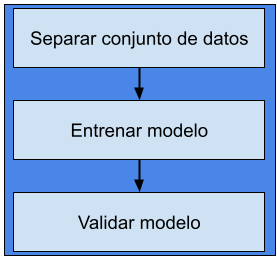
\includegraphics[width=0.5\textwidth]{Metodologia/imgs/DFDefinirModelo.png}
    \caption{Diagrama de flujo para definir un modelo predictivo de la velocidad.}
    \label{fig:ModeloScikitTensorFlow}
\end{figure}

El primer paso es separar el conjunto de datos en un conjunto de entrenamiento y validación. Normalmente esto se realiza en un porcentaje de 70\% (entrenamiento) - 30\% (validación). Una vez separado el conjunto de datos se procede a la optimización de los parámetros del modelo o también llamado entrenamiento. Por último, se utiliza el modelo con el conjunto de validación para validar que los resultados obtenidos.

